% \documentclass[]{amsbook}
\documentclass[]{article}

% \input MyMacros.tex

\usepackage{graphicx}% Include figure files
\usepackage{dcolumn}% Align table columns on decimal point
\usepackage{bm}% bold math
% \usepackage{pictex}%
\usepackage{verbatim} % this is needed for \begin{comment} ... \end{comment}
\usepackage{lscape} % this is needed for occasional landscape figures
\usepackage{amsmath}
% \usepackage{appendix}
% \usepackage{subfigure}
\usepackage{epsfig}
\usepackage{amsfonts}
\usepackage[margin=1.1in, top=1.1in, bottom=1.1in]{geometry}

% \textwidth 550pt
% \textheight 500pt
% \hoffset -3.5cm
\def\betabold{{\pmb{$\beta$}}}

\setcounter{tocdepth}{3}
%
\begin{document}

\date{January 1, 2020}

% \voffset=1.5
\title{
\centerline{}
\centerline{}
\centerline{}
Matching of EDM Prototype Ring Circumference \\
to Injection Ring Circumference
}
\author{R. Talman and J. Talman
}

\maketitle

% \tableofcontents

\begin{abstract}
Pursuant to CERN Yellow Report (CYR) ``Storage Ring to Search
for Electric Dipole Moments of Charged Particles:
Feasibility Study'' this report expands upon Chapter 7 
``The EDM Prototype Ring (PTR)'', with special emphasis
on optimizing the PTR circumference for the injection line beam polarization
preserving filling process.  For concreteness in this report, the COSY ring
(with $\mathcal{C}_{\rm INJ}=182\,$m circumference) is taken as the injection 
ring prototype,
but the methodology can be easily adapted to other circumference choices.
The main issue, to permit single bunch train transfer, is that INJ and PTR
ring circumferences should be related by ``easy'' rational fractions--here,
for INJ/PTR we consider only the fractions 1/2, 3/4, and 1/1. Other
significant issues are availability of free straight section length for 
needed apparatus, required electric field maximum, and overall PTR cost. 
\end{abstract}
%

\section{All-electric ring scaling from the CERN Yellow Report}
\subsection{Initial assumptions}
There has been concern whether or not the PTR ring described in the 
CERN Yellow Report (CYR)\cite{CYR}  
has sufficient total free drift space for required diagnostic and beam handling equipment. 
One approach could be to migrate from rounded-square ring shape to racetrack-shape, to make 
more space available.  I have come to believe that this is a bad idea for two reasons. 

Injection at a corner, as shown in Figure~\ref{fig:PTR-corner-injection}, seems economical 
and ideally symmetric for injecting counter-circulating beams. This symmetry would be lost
in a race-track configuration, complicating the task of exactly matchingh beam profiles.
%
\begin{figure}[htbp]
\centering
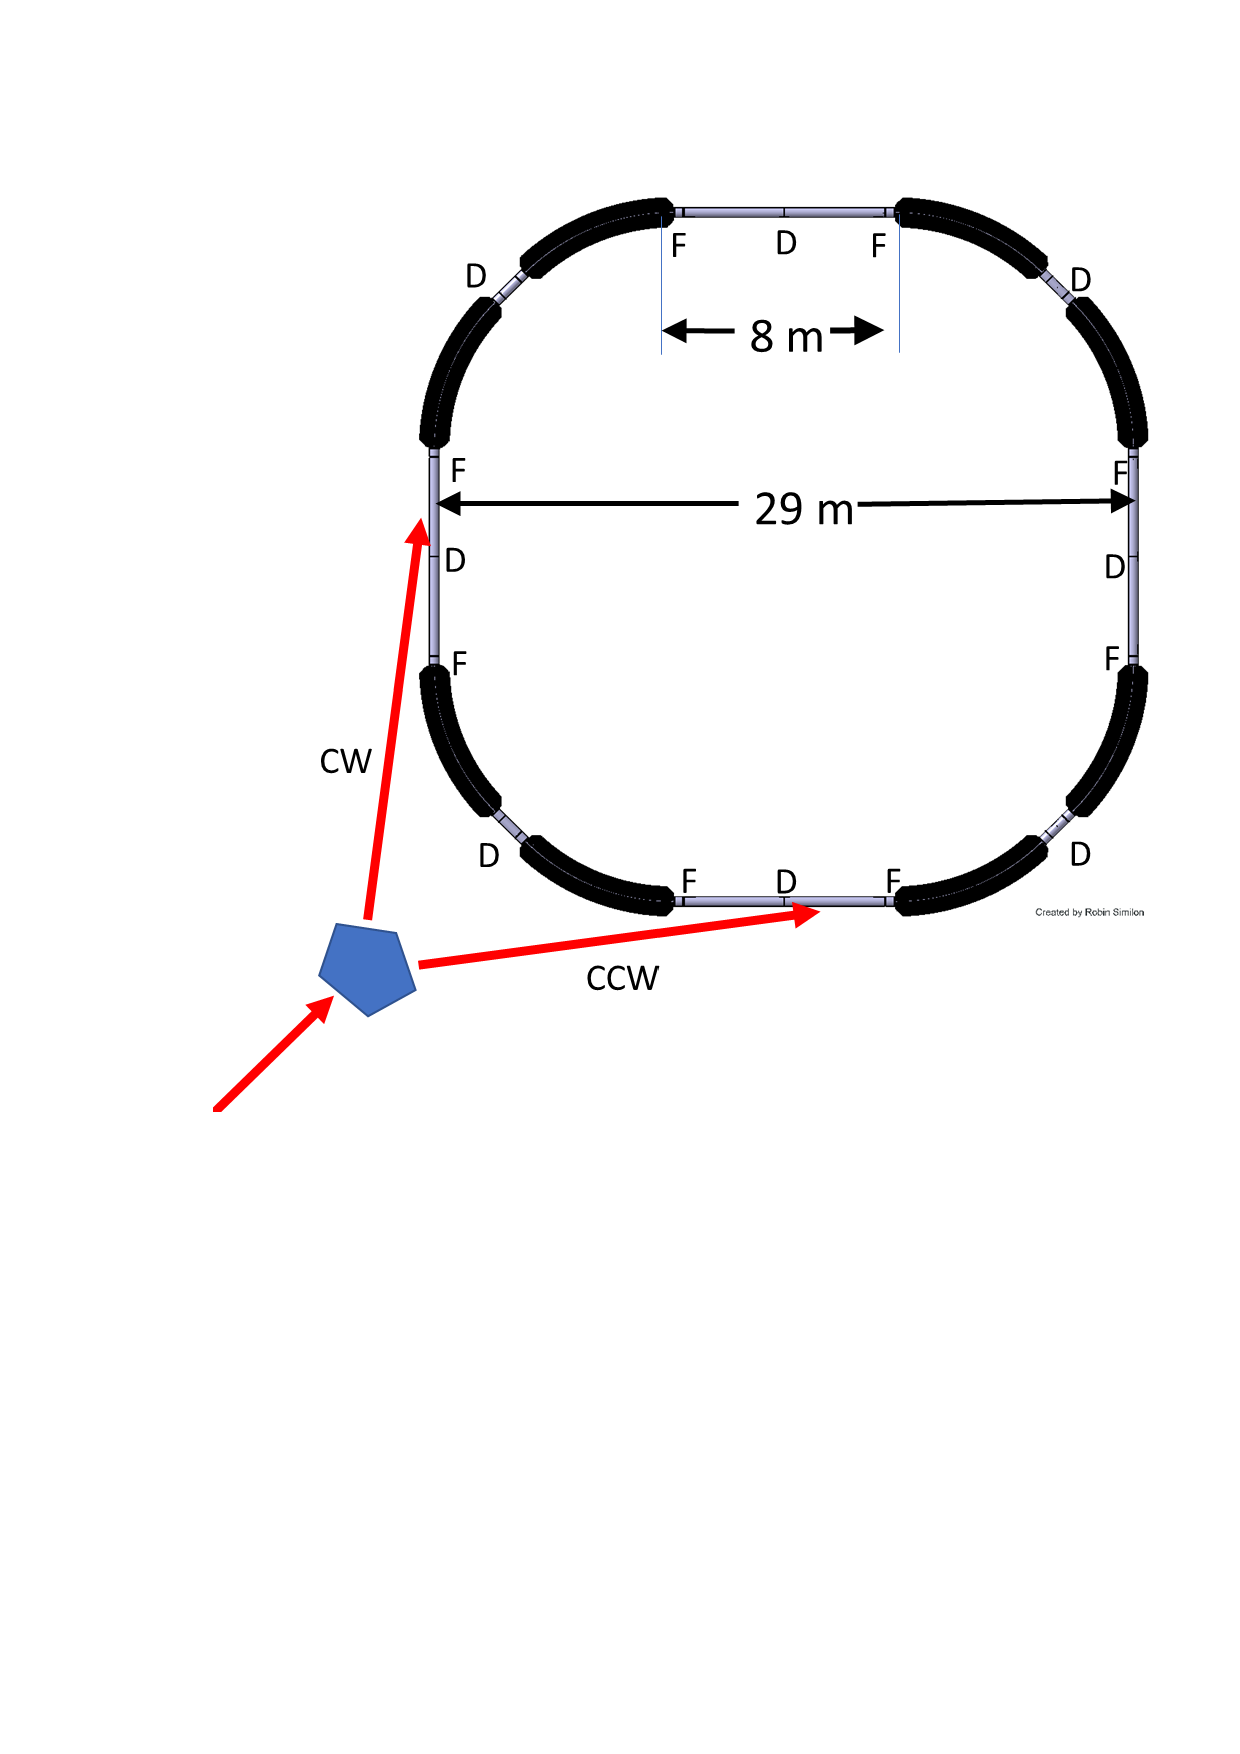
\includegraphics[scale=0.50]{pdf/Fig-4-injection3.pdf}
\caption{\label{fig:PTR-corner-injection}(Copied from CYR) the basic layout of the prototype ring 
consists of 8 dual, superimposed electric and magnetic bends; 2 families of quadrupoles---focusing~(F) 
and de-focusing (D); 
with an optional skew quadrupole family at mid-points of the four 8\,m long straight sections. 
The total circumference, as described in the CYR, was about 100\,m. The three lattices described in
the present report have nominal circumferences of 90.8\,m, 136.5\,m, and 183\,m, intentionally 
(but only approximately, so far) adjusted close to 1/2, 2/3, and 1/1 times the COSY ring circumference. 
Otherwise the ring designs are unchanged from the CYR.} 
\end{figure}
%
A probably more serious problem is that the focusing implied by long straight sections
precludes the possibility of tuning the vertical tune $Q_y$ down close to zero. 
This sacrifices self-magnetometry sensitivity, which scales as $1/Q_y$.

In this report I therefore consider only rounded-square lattice shapes. It is 
convenient that the required ring scaling was already faced in the far greater
range from PTR scale to Holy-Grail scale. I also assume the quadrupoles labeled ``D''
in Figure~\ref{fig:PTR-corner-injection}, and differently in Figure~\ref{fig:pEDM-square-proto},
located at the mid points of long straight sections, will not be needed.

Only three lattices are considered: one with the same circumference as COSY, one
with half-COSY circumference (roughly the same as the CYR-nominal PTR ring) and
one half way between these two cases.
With COSY taken as the choice for INJ, the ideal PTR
circumferences are $\mathcal{C}_{\rm PTR}= 91\,m, 136.5\,m, and 182$\,m;
(with designated file-names identifications
``-0p5-COSY'', ``-0p75-COSY'', and ``-1p0-COSY). 

Furthermore I have chosen to emphasize the (difficult)
low $Q_y$ (high $\beta_y$) region. (As demonstrated in Chapter~7 of the CYR) 
the quite numerous QF and QD quadrupoles provide ample tuning range for both
tunes, $Q_x$ and $Q_y$. The three rings in this report remain (at least nominally)
capable of being tuned down arbitrarily close to the $Q_x=Q_y=0$) limit.  This capability is
provided by altering gradient, very-weakly focusing $m \neq 0$ electrode shaping.  
But, for most ring commissioning, the focusing provided by QF and QD quads will be dominant,
making the electrode shapes, effectively, purely cylindrical (i.e. $m\approx\pm0$).

Focusing on the technically-difficult, low $Q_y$, limit makes the cases addressed
in this report hypersensitive. Strengthening the QF/QD focusing from this limit
can be performed easily.  More technical discussion of these points has already been
given in CYR Chapter~7.

All parameter determinations in this report are based on coordinating two 
entirely different ring design programs. One of these, referred to as ``MAPLE'', is based on 
Wollnik linear transfer matrices, and is essentially equivalent to Valeri Lebedev's similar
program\cite{Lebedev}---traditionally there has been quite good agreement between 
Valeri's and my versions of these explicitly linearized Courant-Snyder codes. 

The other ring design program is referred to as 
``ETEAPOT''\cite{BNL-Electic-Analogue}\cite{ETEAPOT}. Patterned after
TEAPOT\cite{TEAPOT}\cite{TEAPOT2}\cite{TEAPOT3}, developed for the SSC
by Lindsay Schachinger and me, ETEAPOT is based entirely on particle tracking. 
In this approach, ring transfer matrices are calculated 
as outputs rather than being provided analytically as inputs. Traditional lattice parameters, 
such as tunes, Twiss functions, and dispersions, are obtained from the derived transfer maps 
(including higher than linear order, if necessary).

The figures in this report show that agreement between MAPLE and ETEAPOT models, though excellent,
is not perfect. I think the small discrepancy is due to an approximation built into ETEAPOT (which
is nominally exact for $m=1$ electrode shapes, but needs to be exrapolated to the $m=\pm0.002$
(almost exactly ``cylindrical'') design electrode shapes. This extrapolation range is large
enough for its linearity assumption to be questionable. 

This discrepancy remains to be investigated. For now
a single parameter, the same for all three rings, constrains the maximum 
vertical beta function values obtained by MAPLE and ETEAPOT to agree. 
(Compare Figures~\ref{fig:E-PTR2-ETEAPOT-betay} and \ref{fig:E-PTR2-MAPLE-betay},
and accompanying tables, \ref{tbl:0p5}, \ref{tbl:0p75}, and \ref{tbl:1p0},
where the free parameter is indicated a an argument of ETEAPOT[-0.032].)
As a result the vertical beta functions obtained by ETEAPOT differ by as much as
ten percent from those calculated by MAPLE (in the hypersensitive high $\beta_y$ region).
This level of disagreement seems ignorable for the time being. As already mentioned, 
this comparison has been made in the ``fine-tuning limit'' for which the vertical tune
is close to zero.

\subsection{Adjusting PTR design based on CYR ``Holy Grail'' scaling prescription}
This section describes a four parameter lattice design for a complete family of 
stable all-electric storage rings, ranging from the PTR ring at the small radius, 
low energy end, to a full scale, large radius, high energy end. This is the
same prescription, as described in the CYR report, for scaling down from the
``Holy Grail'' design to the nominal  PTR design.
This skeletal PTR prototype lattice design, copied from CYR, 
is shown in Figure~\ref{fig:pEDM-square-proto}. 
\medskip
%
\begin{figure}[hbp]
\centering
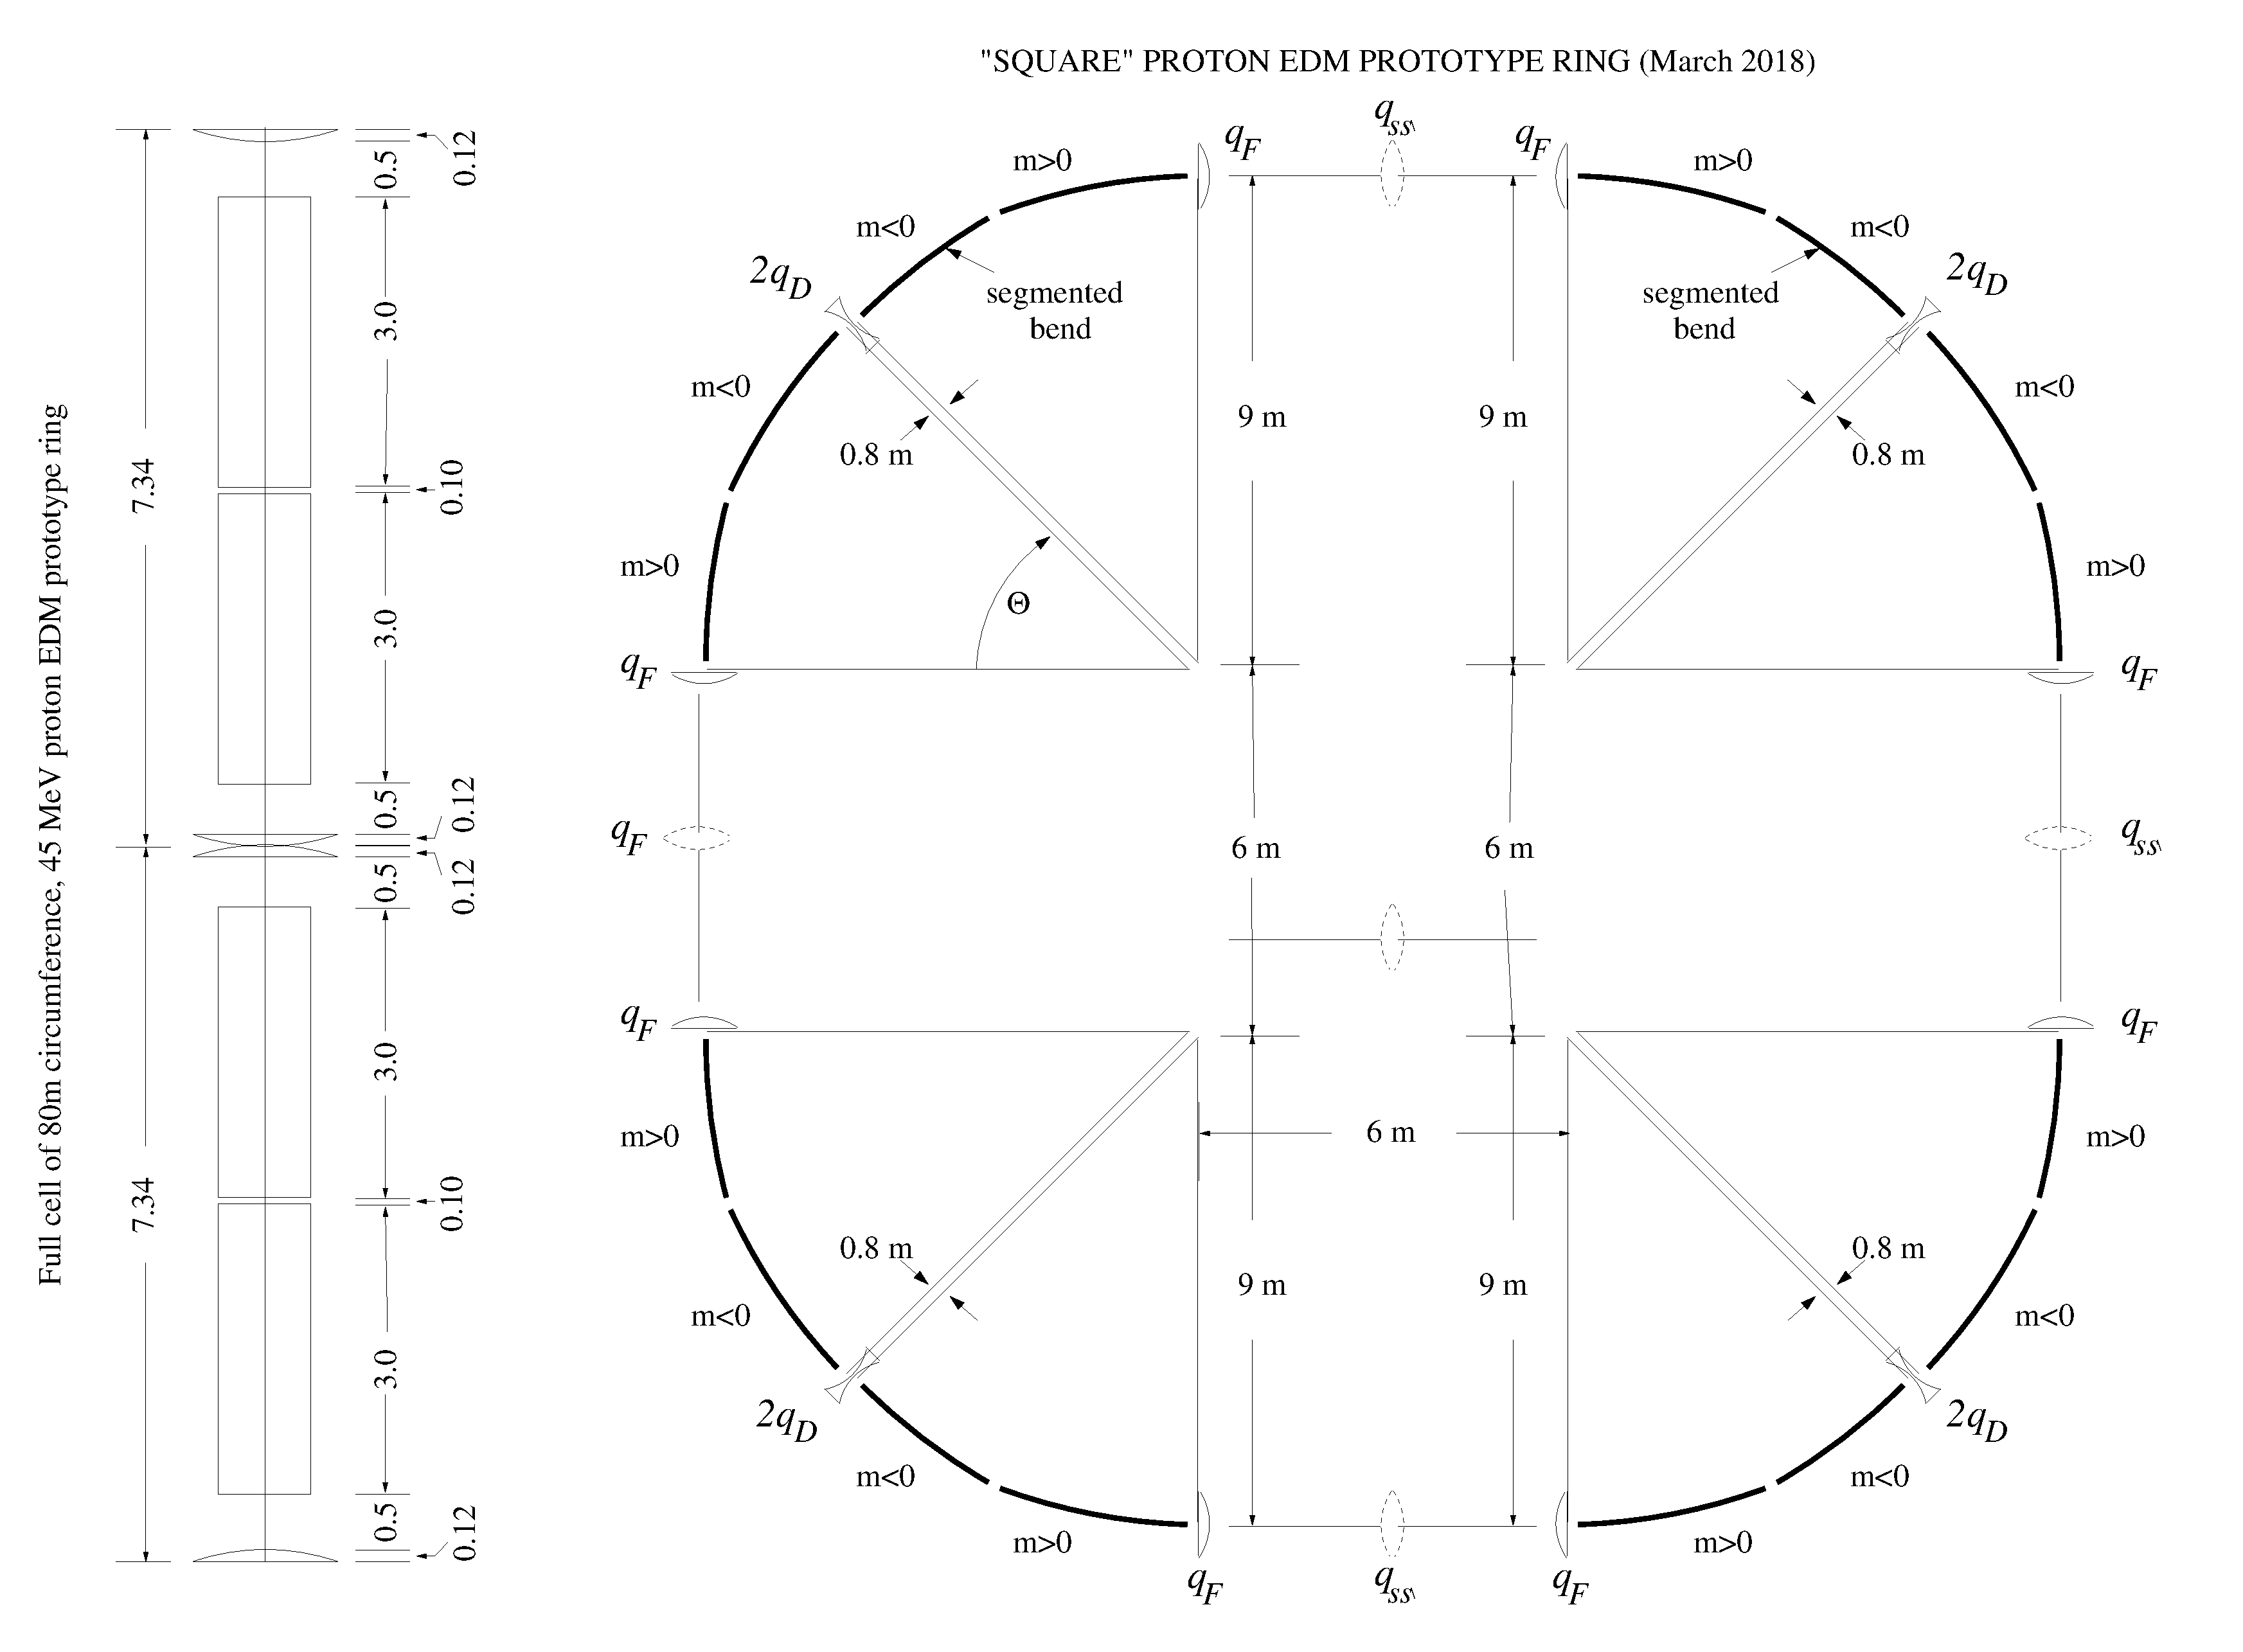
\includegraphics[scale=0.25]{pdf/pEDM-square-proto-w-fullcell.pdf}
\caption{\label{fig:pEDM-square-proto} Lattice layouts for proposed lattice 
half-cell (left) and full 
ring (right). The accumulated drift length is not enough for the ring
to operate ``below transition''.  When scaling up to the eventual, full 
energy, all-electric ring, from four-fold to sixteen-fold symmetry, with
drift lengths and bend lengths preserved (but bend angles four times less)
the total circumference is to be about 500\,m and operation will be well
below transition.} 
\end{figure}
%
In all considered ring designs, for flexibility, focusing is provided both
by separated-function electric quadrupoles, and by (very weak) 
alternating-gradient, combined-function, electrode-shape focusing.
The designs in this report assume extremely weak electrode-shape 
focusing but with predominently lumped quadrupole focusing for routine 
operations. 

The scaling in the present report uses the scaling prescription
explained in the CYR, which introduced a four-parameter family of
all-electric rings.  The four parameters for the rings in that report are
exhibited in the upper table of Table~\ref{tbl:MagicScaling}. A corresponding
table for the present report is exhibited in the ower table of 
Table~\ref{tbl:MagicScaling}. By introducing the ratio 
$\rho_{\rm L/R}$=L\_LONG\_STRAIGHT/R\_NOMINAL$\approx0.6$, also shown in the lower table,
it can be seen that, over the smaller range of bending radii considered in this
report, the number of free parameters needed is (roughly) reduced from four to three.
%
\begin{table}[hbp] \scriptsize
\caption{\label{tbl:MagicScaling}(Copied from CYR)
the four major parameters for scaling between full scale ring and prototype ring.
They describe a continuum of stable, all-electric storage rings ranging from small, 
low energy to large, high energy. Their uppercase names make these parameters easily 
recognizable in lattice description files. The remaining (minor) parameters are
given in Table~\ref{tbl:MagicScaling.2}.} The upper table (copied fro CYR) gives
parameters approptiate for variable proton energy. The lower table (specific to this report) 
gives parameters for variable PTR circumference.
\vskip 0.2cm
\centering
\begin{tabular}{|l|c|ccc|c|}  \hline
parameter           & E\_30MeV & EM\_35MeV & EM\_45MeV & EM\_55MeV & E\_233MeV \\ \hline
  R\_NOMINAL [m]      &   9.0    &   9.0     &    9.0    &   9.0     &    40.0   \\
L\_LONG\_STRAIGHT [m] &   6.0    &   6.0     &    6.0    &   6.0     &    14.8   \\ 
   N\_SUPER           &    4     &    4      &     4     &    4      &    16     \\
   M\_NOMINAL         &   0.1    &   0.1     &    0.1    &   0.1     &    0.1    \\ 
 \hline
\end{tabular}
\vskip 0.5cm
\centering
\begin{tabular}{|l|ccc|}  \hline
parameter             & E-PTR2-0p5-COSY         & E-PTR2-0p75-COSY         &  E-PTR2-1p0-COSY        \\ \hline
  R\_NOMINAL [m]      &     10.0                &     15.4                 &      21.0               \\
L\_LONG\_STRAIGHT [m] &  6.00=0.60 x R\_NOMINAL &  8.932=0.58 x R\_NOMINAL & 11.76=0.56 x R\_NOMINAL \\ 
   N\_SUPER           &       4                 &       4                  &        4                \\
   M\_NOMINAL         &    $\pm$0.002           &    $\pm$0.002            &   $\pm$0.002            \\ 
 \hline
\end{tabular}
\end{table}
%
(For variation over the full PTR to ``Holy Grail'' range, 
the adopted scaling relations follow: the field index scales inversely with 
super-periodicity N\_SU\-PER; with $m=\pm$M\_NOMINAL being the field indices of the 
prototype ring, the scaling relation is $m=\pm$M\_NOMINAL*4/N\_SUPER. 
Lattice names are in the column headings. 
Minor (unchanged) parameter valus are indicated in Table~\ref{tbl:MagicScaling.2}, which has
also been copied, unchanged, from the CYR.
%
\begin{table}[h] \scriptsize
\caption{\label{tbl:MagicScaling.2}(Copied from CYR, and unchanged for this report,) 
minor geometric parameters: Theta, $r0$, 
$leh$, $lss=0.8$\,m, and $llsh$ are, respectively, bend/half-period, bend radius, 
bend-half-length, short-straight-length, and long-straight-half-length. 
$K0$ is proton kinetic energy and $\pm m_{in}$ are alternating field index values.
Minor kinetic parameters: $lq$ is quad length, $qF$ and
$qD$ are quad strengths, $gBy2$ is half-gap width, $Q_x$ and $Q_y$ are tunes.
}
\centering
\begin{tabular}{|l|cccccc|ccccc|}  \hline
lattice name &    K0    &  m\_in  &  Theta &  r0  & leh  & llsh &   lq    &   qF/qD     &  circ. &  gBy2   &   Q\_x/Q\_y \\
             &  [MeV]   &         &    [r] & [m]  & [m]  &  [m] &   [m]   &   [1/m]     &   [m]  &   [m]   &              \\ \hline
E\_30MeV     &  0.0300  &  0.100  &  0.785 &  9   & 3.53 & 2.60 &  0.2000 & $\mp0.01$   & 83.7   &  0.035  &  1.768/0.093 \\  \hline
EM\_45MeV    &  0.0450  &  0.100  &  0.785 &  9   & 3.53 & 2.60 &  0.2000 & $\mp0.01$   &  83.7  &  0.035  &  1.750/0.093 \\ \hline
E\_233MeV    &  0.2328  &  0.025  &  0.196 & 40   & 3.93 & 7.00 &  0.2000 & $\mp0.0025$ &  501   &  0.015  &  1.815/0.145 \\  \hline
\end{tabular}
\end{table}
%

(For what seems like the most promising ``three-quarters COSY'' case)
detailed lattice descriptions (needed for computer processing) 
are contained in the following files (which supercede the
corresponding files referenced in CYR, are are also available on request).
Since the first two of these files are quite short (yet provide a complete idealized lattice 
description and are easily humanly-decipherable) they are attached as appendices to this report.
The remaining two files, produced by XSLT software, merge the first two files into long,
computer readable files that need to be readable by human beings only for debugging purposes.

\begin{description}
\item{{\bf\tt E-PTR2-0p75-COSY-con\_xml}:  }
``{\tt .xml}'' file containing 
all parameters (both symbols and their values) for a small 
proton EDM prototype ring, including (symbolic) 
parameters for scaling to the large (500\,m circumference) all-electric 
proton EDM ring.
\item{{\bf\tt E-PTR2-0p75-COSY-nocon\_xml}:  }
Symbolic ``{\tt .xml}'' file describing the idealized lattice design. (Actually
this file does not depend on ring radius--it is therefore 
identical to {\bf\tt E-PTR2-0p5-COSY-nocon\_xml} and {\bf\tt E-PTR2-1p0-COSY-nocon\_xml}). 
\item{{\bf\tt E-PTR2-0p75-COSY.adxf}:  }
Numerical ``{\tt .adxf}'' file describing idealized lattice design.
\item{{\bf\tt E-PTR2-0p75-COSY.sxf}:  }
Numerical ``{\tt .sxf}'' file describing fully-instantiated lattice design
(though without differentiated (i.e. individualized) parameter values.)
\end{description}
%
Initially, for both prototype and full-scale ring, the horizontal tune
was expected to be just below 2.0 and the vertical tune much less than 1.0,
and tuneable to a value as low as 0.02. The
ultra-low vertical tune requirement is needed to reduce the
vertical restoring force, therby enhancing the beam ``self-magnetometry'' 
sensitivity to beam displacement caused by radial magnetic field. 

(As an aside, it can now be mentioned, that the doubly-magic EDM 
measurement method possibility avoids the need for ultraweak vertical 
focusing, allowing the focusing to be much stronger than was initially anticipated.
A very thorough and valuable 2015 study by V. Lebedev\cite{Lebedev} analysed 
two frozen-spin all-electric designs, one very weak-focusing, the other 
stronger focusing. With ultra-low vertical tune no longer necessary, the
scaled down PTR can be said to more nearly correspond to
the stronger-focusing ring Valeri favoured.)

For the full-scale ring the correspondingly smaller tune advance per 
super-period causes the focusing to be weaker. This is what 
permits the long straight sections of the full scale ring to be almost
doubled, compared to the prototype (from 6\,m to 14.8\,m). 
This has the beneficial (perhaps even obligatory) effect, for the full-scale ring, 
of operating ``below transition''. This ameliorates intrabeam scattering, 
as can be explained in connection with stochastic cooling. 
(Conversely, this is one respect in which the prototype ring optics still is a 
not-quite-faithful prototype.) This choice was made to reduce the prototype 
size.

\section{Determination of Twiss Functions From Transfer Matrices}
Like the magnetic accelerator simulation code TEAPOT, the electric accelerator
code ETEAPOT, does not base particle tracking on theoretically-derived
transfer matrices. Rather, a standard set of small amplitude particles are 
tracked (i.e. to satisfy Newton's force law). Then, by differencing the outputs,
transfer matrices are extracted---in what amounts to numerical differentiation.
Then, from the transfer matrices, the lattice twiss functions are derived. Because
this is an unconventional approach, the following sections explain the approach
in more detail.

\subsection{Analysis of the Once-Around Transfer Matrix at the Origin}
In this section $x$ and $y$ and $ct$ subscripts will be suppressed,
and only transverse evolution is to be discussed. 
The most general
transfer matrix is a six-by-six matrix ${\bf M}(s_i,s_j)$, which propagates a
phase space vector ${\bf x}(s_i)$ at $s_i$, to its value ${\bf x}(s_j)$ at $s_j$;
%
\begin{equation}
{\bf x}(s_j) 
 =
{\bf M}(s_i,s_j)\,
{\bf x}(s_i). 
\label{TM.1}
\end{equation}
%
ETEAPOT starts by assigning coordinates at the origin, $s_0=0$,
to the particles in a standard bunch (as described earlier), and then
evolves the standard bunch and records the coordinates ${\bf x}(s_i)$ 
at all points $s_i$.  From these results the transfer matrices 
${\bf M}(0,s_i)$ can be calculated (also as described earlier). By definition
%
\begin{equation}
{\bf M}(0,0)
 =
{\bf I}, 
\label{TM.2}
\end{equation}
%
where ${\bf I}$ is the $6\times6$ identity matrix. 

To extract Twiss lattice functions one needs periodic, ``once-around'' transfer 
matrices, distinguished by overhead tildes, and defined by
%
\begin{equation}
{\widetilde{\bf M}}(s_i)
 \equiv
{\bf M}(s_i,s_i+\mathcal{C}_0)
 =
{\bf M}(0,s_i)\,
{\bf M}(s_i,\mathcal{C}_0).
\label{TM.3}
\end{equation}
%
where $\mathcal{C}_0$ is the circumference of the design
orbit; the final step has been taken because knowledge of
$s_i+\mathcal{C}_0$ requires tracking for more than one
complete turn, but we are assuming that tracking has been
done only for exactly one complete turn. Propagation from
$s=\mathcal{C}_0$ to $\mathcal{C}_0+s_i$ is the same as
propagation from $s=0$ to $s_i$. The Twiss parameterization of 
(one partitioned diagonal
$2\times2$ block of) such a once-around, symplectic 
transfer matrix is
%
\begin{equation}
{\widetilde{\bf M}}(s_i)
 =
\begin{pmatrix}
\cos\mu + \alpha\sin\mu          & \beta\sin\mu \\
-\frac{1+\alpha^2}{\beta}\sin\mu & \cos\mu - \alpha\sin\mu 
\end{pmatrix}.
\label{TM.4}
\end{equation}
%
Extraction of the $\alpha_0$ and $\beta_0$, the Twiss parameters 
at the origin, can start from
%
\begin{equation}
\cos\mu
 = 
\frac{1}{2}\,\big({\widetilde{\bf M}}_{11}(0) + {\widetilde{\bf M}}_{22}(0)\big),
\label{TM.5}
\end{equation}
%
which fixes $\cos\mu$. Because of sign ambiguity, this determines only
$|\sin\mu|$. One also has the relations
%
\begin{equation}
\beta_0
 = 
\bigg|
\frac{\widetilde{\bf M}_{12}(0)}{\sin\mu}
\bigg|.
\label{TM.6}
\end{equation}
%
and
%
\begin{equation}
\alpha_0
 = 
\frac{1}{2\sin\mu}\,
\big({\widetilde{\bf M}}_{11}(0) - {\widetilde{\bf M}}_{22}(0)\big).
\label{TM.7}
\end{equation}
%
With $\beta$ being positive by convention, 
from the 1,2 element, sign($\sin\mu$) can be seen to be
the same as sign(${\widetilde{\bf M}}_{12}$). With $\cos\mu$ known,
this fixes $\sin\mu$.
Together, these relations fix $\sin\mu$, $\cos\mu$, $\alpha_0$, and $\beta_0$.

Conventionally one also introduces a third Twiss parameter
%
\begin{equation}
\gamma_0
 = 
\frac{1+\alpha_0^2}{\beta_0},
\label{TM.8}
\end{equation}
%
which can be obtained once $\beta_0$ and $\alpha_0$
have been determined. 

Because of the multiple-valued nature of inverse trig functions,
these relations do not determine a unique value for $\mu$. They do,
however, determine the quadrant in phase space in which the angle $\mu$
resides. For sign($\sin\mu$)$>$0 the angle $\mu$ resides in the first
or second quadrant, in which case the fractional tune is less than 1/2;
otherwise the fractional tune is greater than 1/2.
For sign($\cos\mu$)$>$0 the angle $\mu$ resides in the first
or fourth quadrant, in which case the fractional tune is below 1/4
or above 3/4. These considerations fix the fractional parts of
the tunes.

An ``aliasing'' or ``integer-tune'' ambiguity remains, however,
which cannot, even in principle, be obtained from the once-around 
matrix. Only if both transverse tunes are less than 1 (which is 
hardly ever the
case) would the tunes be equal to the fractional tunes that have
been determined. In general, to obtain the integer tunes, it is 
necessary to analyse the turn by turn data at sufficiently closely-space 
intermediate points in the lattice.

\subsection{Evolving the Twiss Functions Around the Ring}
To find the Twiss parameters at an arbitrary location $s_i$ in the
ring requires the once-around transfer matrix ${\widetilde{\bf M}}(s_i)$. 
This can obtained most compactly by multiplying the equation
%
\begin{equation}
{\bf M}(0,s_j)
 =
{\bf M}(s_i,s_j)\,{\bf M}(0,s_i)
\label{TM.9}
\end{equation}
%
on the right by ${\bf M}^{-1}(0,s_i)$ to produce
%
\begin{equation}
{\bf M}(s_i,s_j)
 =
{\bf M}(0,s_j)\,{\bf M}^{-1}(0,s_i).
\label{TM.10}
\end{equation}
%
Substituting this with $s_j=\mathcal{C}_0$ into Eq.~(\ref{TM.3}) 
produces
%
\begin{equation}
\widetilde{\bf M}(s_i)
 =
{\bf M}(0,s_i)\,\widetilde{\bf M}(0)\,{\bf M}^{-1}(0,s_i).
\label{TM.11}
\end{equation}
%
Having obtained ${\widetilde{\bf M}}(s_i)$,
the procedure described in the previous subsection can
then be used to obtain $\alpha(s_i)$ and $\beta(s_i)$.
But the integer tune ambiguity can, again, not be
resolved. To resolve this ambiguity both $x$ and $y$ phases
have to be tracked continuously through the lattice,
requiring that they advance continuously and monotonically.
(Later, at least in principle, the same ambiguity will 
have to be faced for longitudinal motion. But the
integer longitudinal tune is almost always zero, so the
problem is usually absent in the longitudinal case.)

ETEAPOT requires the lattice description to be in the form
of an {\tt .sxf} file.  To be ``legal'' the granularity of such
a file has to be fine enough that no phase can advance by more
than a quarter integer through any element in the file. Before
working out the $\alpha$ and $\beta$ function evolution, 
ETEAPOT first works out the total phase advances from
the origin to every node specified by the {\tt .sxf} file
(or, if some elements are sliced more finely, by every node
after slicing). 

There is an alternative way of finding the betatron phase
advances. It starts with a Twiss parameterization
of ${\bf M}(0,s)$ from the origin to an arbitrary position $s$
in the lattice;
%
\begin{equation}
{\bf M}(0, s)
 =
\begin{pmatrix}
\sqrt{\frac{\beta(s)}{\beta_0}}\Big(\cos\psi(s) + \alpha_0\sin\psi(s)\Big) & 
            \sqrt{\beta_0\beta(s)}\,\sin\psi(s)                         \\
   \cdot & 
\sqrt{\frac{\beta_0}{\beta(s)}}\Big(\cos\psi(s) - \alpha(s)\sin\psi(s)\Big)         
\end{pmatrix}.
\label{TM.15}
\end{equation}
%
The 2,1 element is quite complicated; it is not shown here since it will not be needed
for the following analysis. Dividing the 1,1 element by the 1,2 element produces
%
\begin{equation}
\frac{{\bf M}_{1,1}(0, s)}{{\bf M}_{1,2}(0, s)}
 =
\frac{\sqrt{\frac{\beta(s)}{\beta_0}}\Big(\cos\psi(s) + \alpha_0\sin\psi(s)\Big)}
     {\sqrt{\beta_0\beta(s)}\,\sin\psi(s)}
 =
\frac{\cot\psi(s) + \alpha_0}{\beta_0}.
\label{TM.16}
\end{equation}
%
Rearranging this equation produces
%
\begin{equation}
\psi(s)
 = 
\tan^{-1}\,
\frac{{\bf M}_{1,2}(0, s)}
     {\beta_0{\bf M}_{1,1}(0, s) - \alpha_0{\bf M}_{1,2}(0, s)}.
\label{TM.17}
\end{equation}
%
Like all inverse trigonometric formulas, this equation has multiple solutions.
But, with the {\tt .sxf} granularity being required to be fine enough, one
can (in principle) sequentially obtain unique phases. With
$\psi(s)$ starting from $\psi(0)=0$, as $s$ increases
from $s_i$ to $s_{i+1}$ there is a unique solution of Eq.~(\ref{TM.17}),
$\psi(s_i)\ge\psi(s_{i-1})$ such that the function $\psi(s)$ increases 
monotonically, as required.
Because the interval from $s_{i=1}$ to $s_i$ is non-zero, $\psi$ will,
superficially, advance discontinuously; the correct solution is the least
discontinuous. The same calculation has to be done for both the $x$ 
and $y$ betatron sectors. 
Unfortunately, even though, theoretically, the phase advances 
monotonically, numerical errors can cause Eq.~(\ref{TM.17}) to
give local phase decrease.  This can cause 
Eq.~(\ref{TM.17}) to give occasionally erratic results.

\section{Tuning-up variable-circumference PTR properties}
Figures~\ref{fig:E-PTR2-ETEAPOT-betax} and 
        \ref{fig:E-PTR2-MAPLE-betax}
compare $\beta_x$ evaluations for the three lattices studied
for this report. Of the rings in this report, {\tt E-PTR2-0p5} is the 
one closest to the prototype ring described in the CERN Yellow Report. 
The alternating gradient pole shape
focusing, though ultraweak, by itself, barely produces vertical stability.
``Geometric'' focusing, though also not very strong, is capable of
providing much stronger horizontal focusing, with horizontal tune $Q_x$
greater than 1.0. For the following graphs, the
QF and QD quads, arranged in FODO pattern, provide stronger focusing
in both planes. As described in CYR, by strengthening QF and QD, there is a large 
tuning range over which $Q_y$ can smoothly increase from barely above 0 to just below 1,
and $Q_x$ can smoothly decrease from barely below 2 to just above 1.   
The figure on the left is evaluated by ETEAPOT, the one on the right by linearized (Wollnik) 
formulas.

There is good qualitative agreement between MAPLE and ETEAPOT.
Quantitative agreemen is not perfect though. This is at least partly
due to a significantly large ``perturbative'' correction from the 
$m=1$ electrode-shape focusing ``Mu\~noz-Pavic'' limit in which ETEAPOT is analtically
exact, to the $m\approx0$ ``cylindrical'' electrode case, aplicable in this,
and all other rings in this report. Side-by-side horizontal beta function comparisons 
are exhibited in Figures~\ref{fig:E-PTR2-ETEAPOT-betax} and \ref{fig:E-PTR2-MAPLE-betax}.
Vertical beta function comparisons are exhibited in Figures~\ref{fig:E-PTR2-ETEAPOT-betay} 
and \ref{fig:E-PTR2-MAPLE-betay}. Horizontal dispersion suctions are shown in
Figure~\ref{fig:E-PTR2-MAPLE-dispersion} and betatron tune accumuation plots are 
shown in Figure~\ref{fig:E-PTR2-MAPLE-TuneAdvance}.

Along with other parameters, much the same lattice function information is shown in 
compressed tabular form in the tables shown right after the figures; 
Table~\ref{tbl:0p5}, ~\ref{tbl:0p75}, and ~\ref{tbl:1p0},
%
\begin{figure}[htbp]
%
\begin{minipage}[b]{0.5\linewidth}
\centering
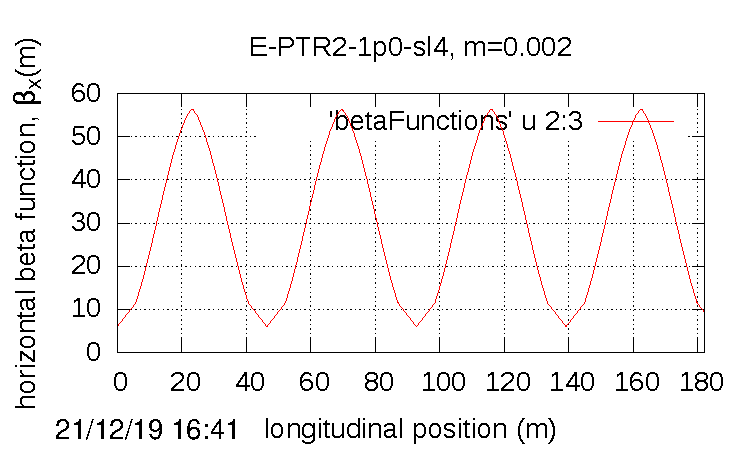
\includegraphics[scale=0.67]{pdf/E-PTR2-1p0-COSY-sl4-Fig_II-9-ETEAPOT.pdf}
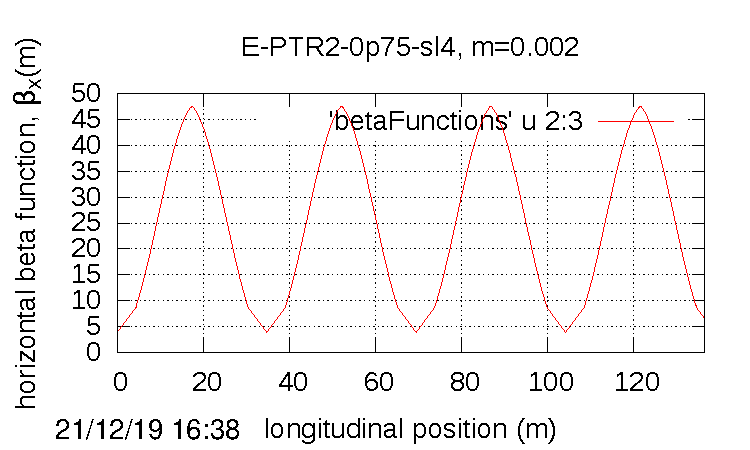
\includegraphics[scale=0.67]{pdf/E-PTR2-0p75-COSY-sl4-Fig_II-9-ETEAPOT.pdf}
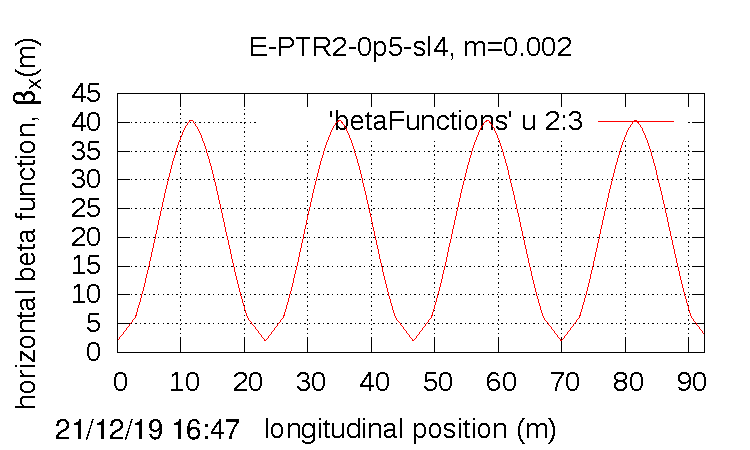
\includegraphics[scale=0.67]{pdf/E-PTR2-0p5-COSY-sl4-Fig_II-9-ETEAPOT.pdf}
\caption{$\beta_x(s)$ calculated by ETEAPOT 
for the {\tt E-PTR2} rings.}
\label{fig:E-PTR2-ETEAPOT-betax}
\end{minipage}
%
%
\begin{minipage}[b]{0.49\linewidth}
\centering
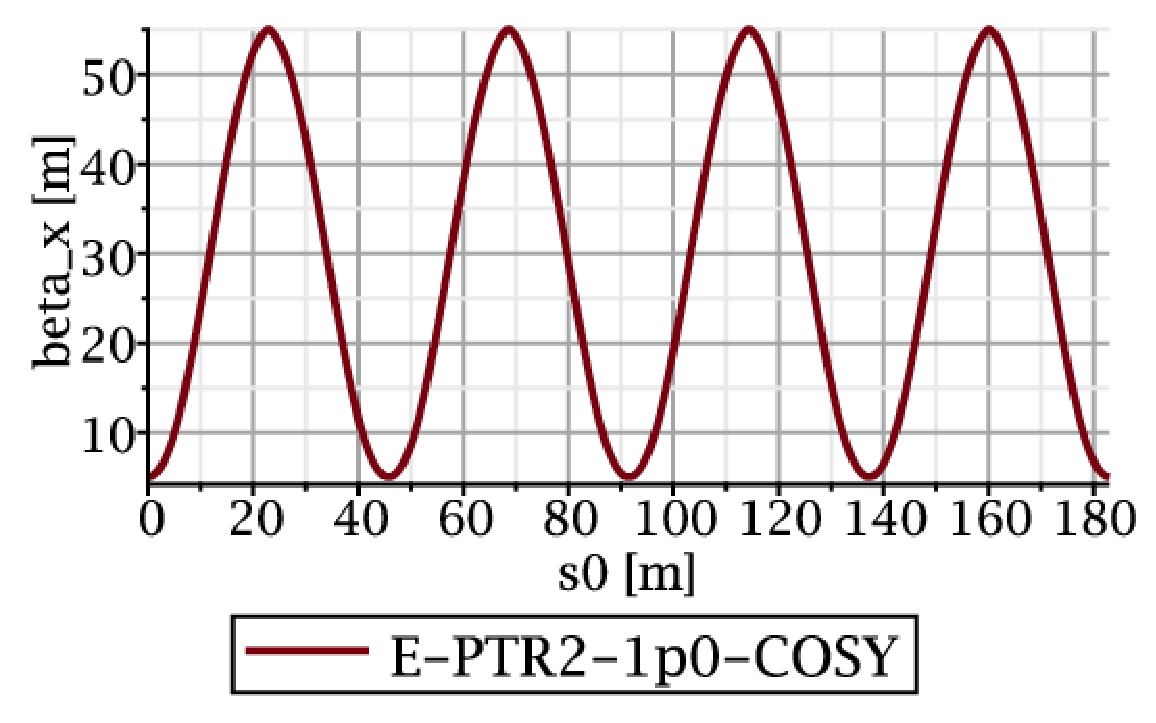
\includegraphics[scale=0.40]{pdf/E-PTR2-1p0-COSY-MAPLE-betax.pdf}
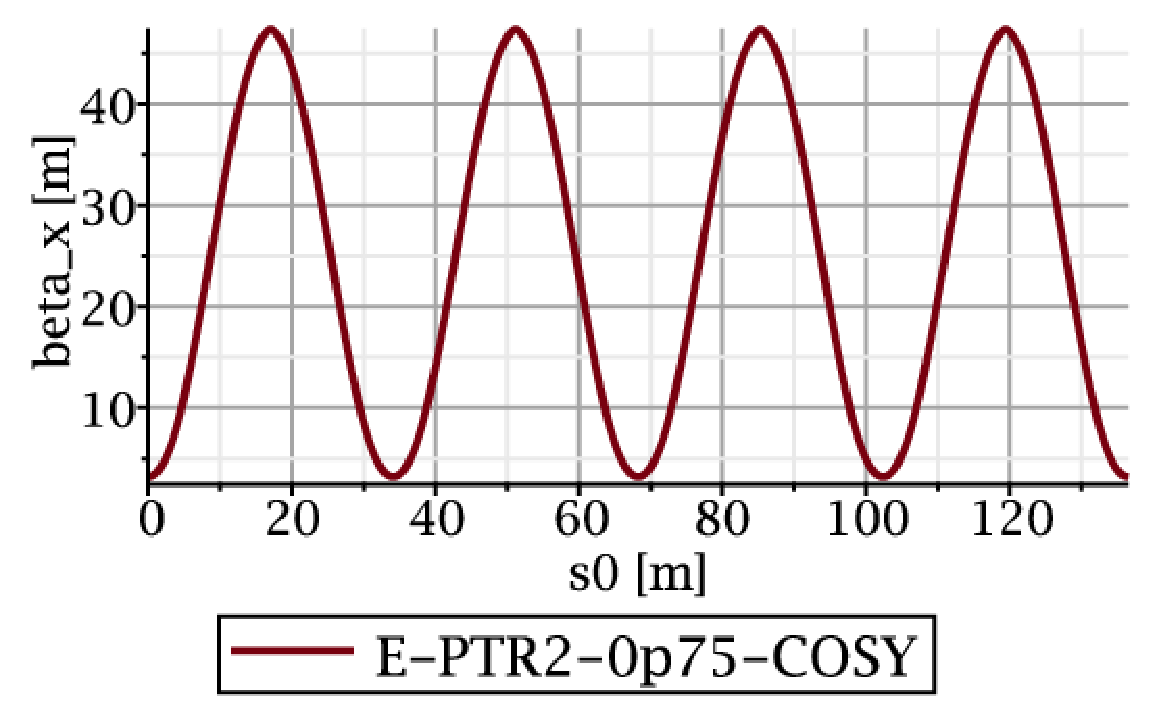
\includegraphics[scale=0.40]{pdf/E-PTR2-0p75-COSY-MAPLE-betax.pdf}
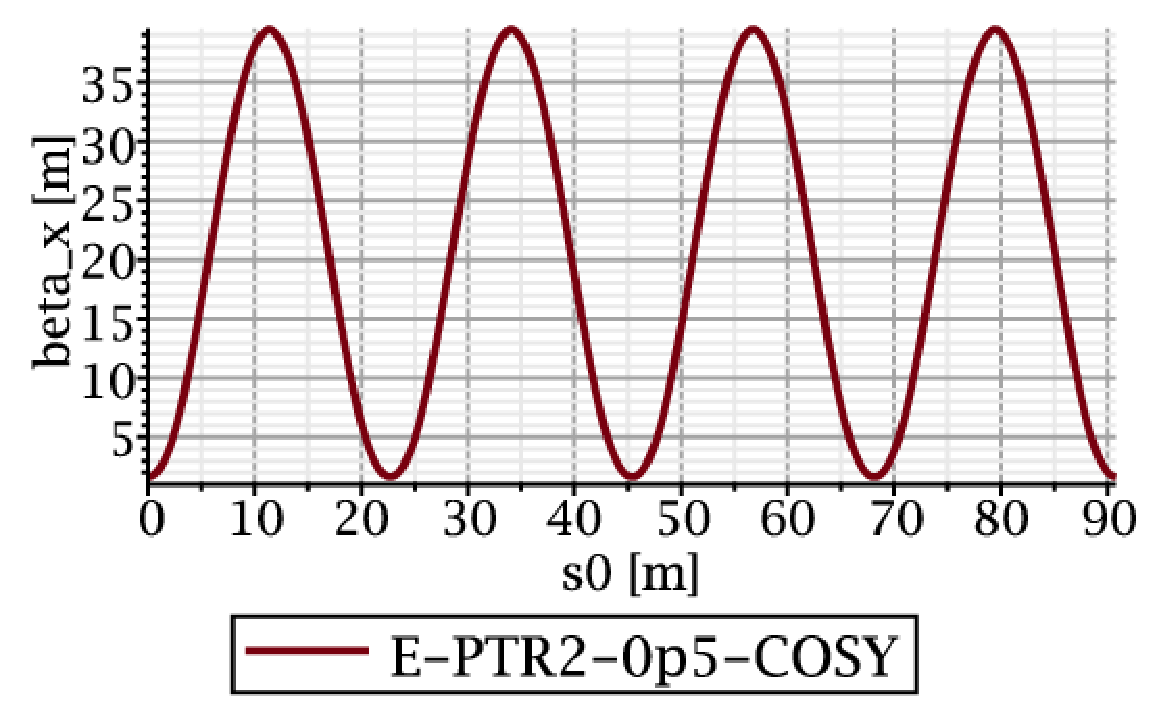
\includegraphics[scale=0.40]{pdf/E-PTR2-0p5-COSY-MAPLE-betax.pdf}
\caption{$\beta_x(s)$ calculated by MAPLE linearized 
theory for the {\tt E-PTR2} rings.}
\label{fig:E-PTR2-MAPLE-betax}
\end{minipage}
\end{figure}
%
%
\begin{figure}[htbp]
\hspace{-0.6cm}
\begin{minipage}[b]{0.45\linewidth}
\centering
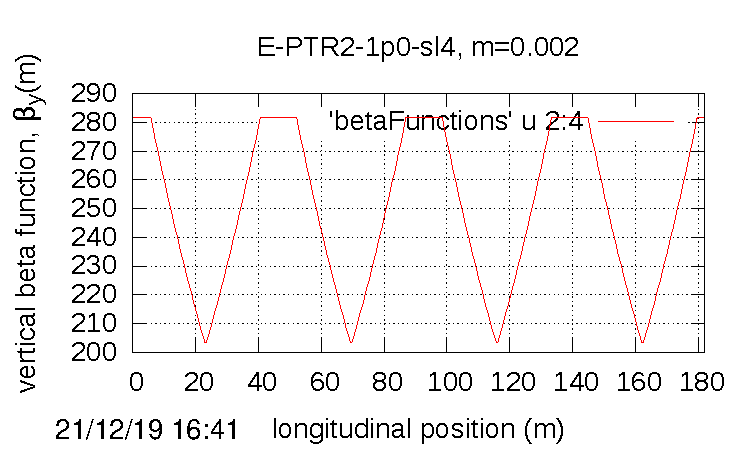
\includegraphics[scale=0.67]{pdf/E-PTR2-1p0-COSY-sl4-Fig_II-11-ETEAPOT.pdf}
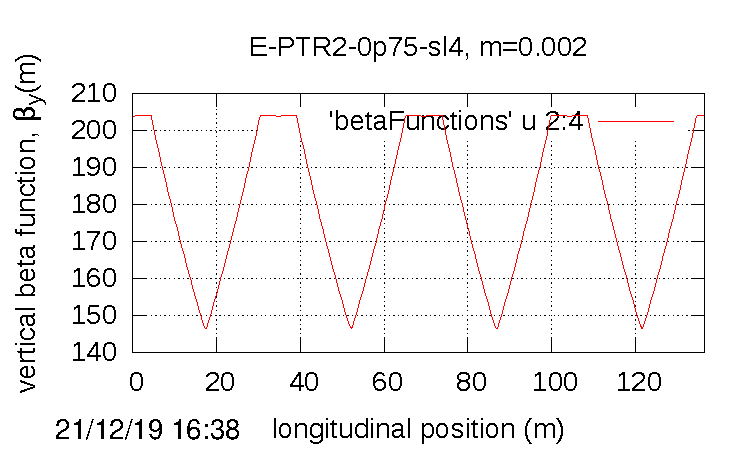
\includegraphics[scale=0.67]{pdf/E-PTR2-0p75-COSY-sl4-Fig_II-11-ETEAPOT.pdf}
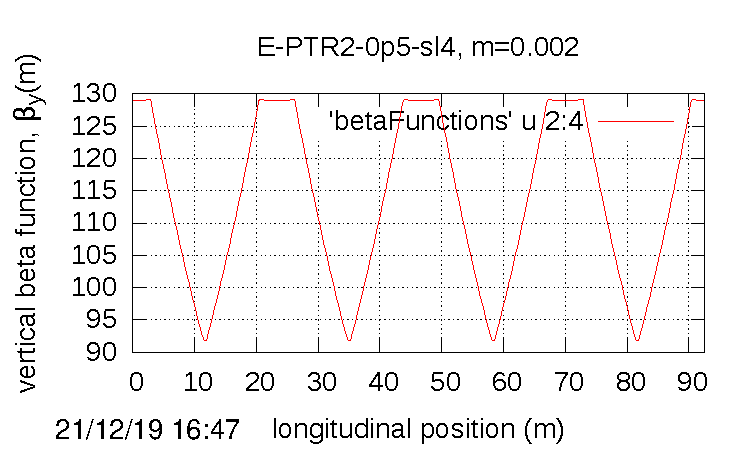
\includegraphics[scale=0.67]{pdf/E-PTR2-0p5-COSY-sl4-Fig_II-11-ETEAPOT.pdf}
\caption{$\beta_y(s)$ calculated by ETEAPOT the {\tt E-PTR2} rings.}
\label{fig:E-PTR2-ETEAPOT-betay}
\end{minipage}
%
%
\begin{minipage}[b]{0.45\linewidth}
\centering
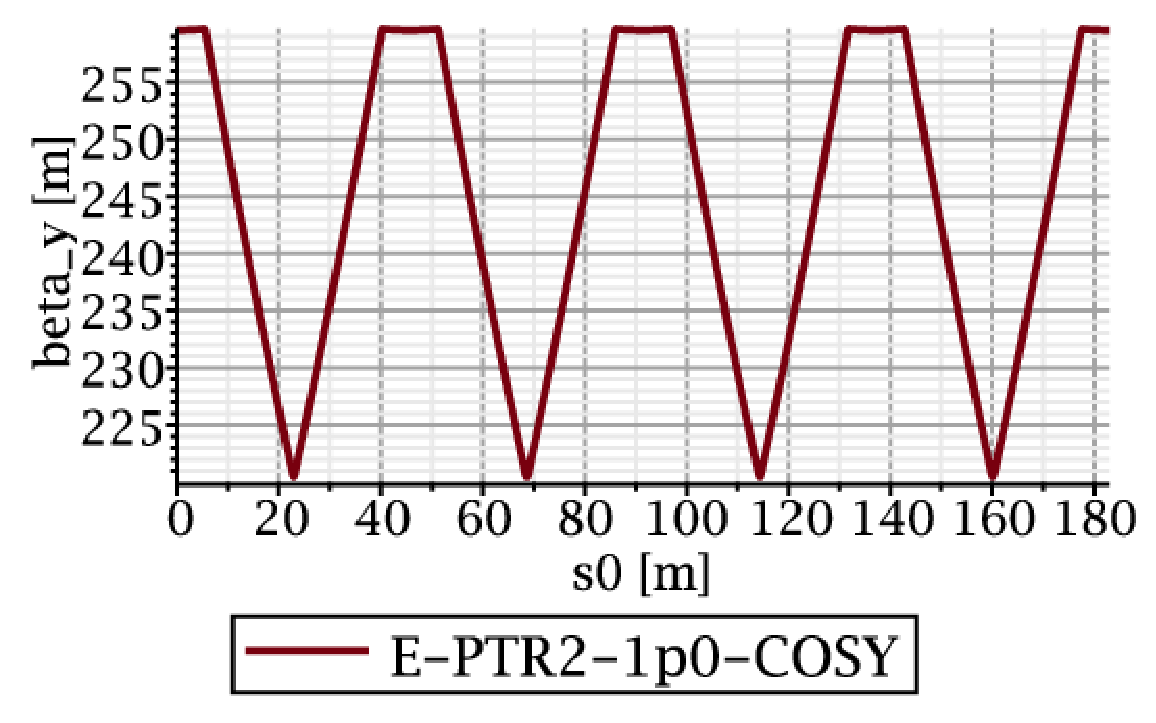
\includegraphics[scale=0.40]{pdf/E-PTR2-1p0-COSY-MAPLE-betay.pdf}
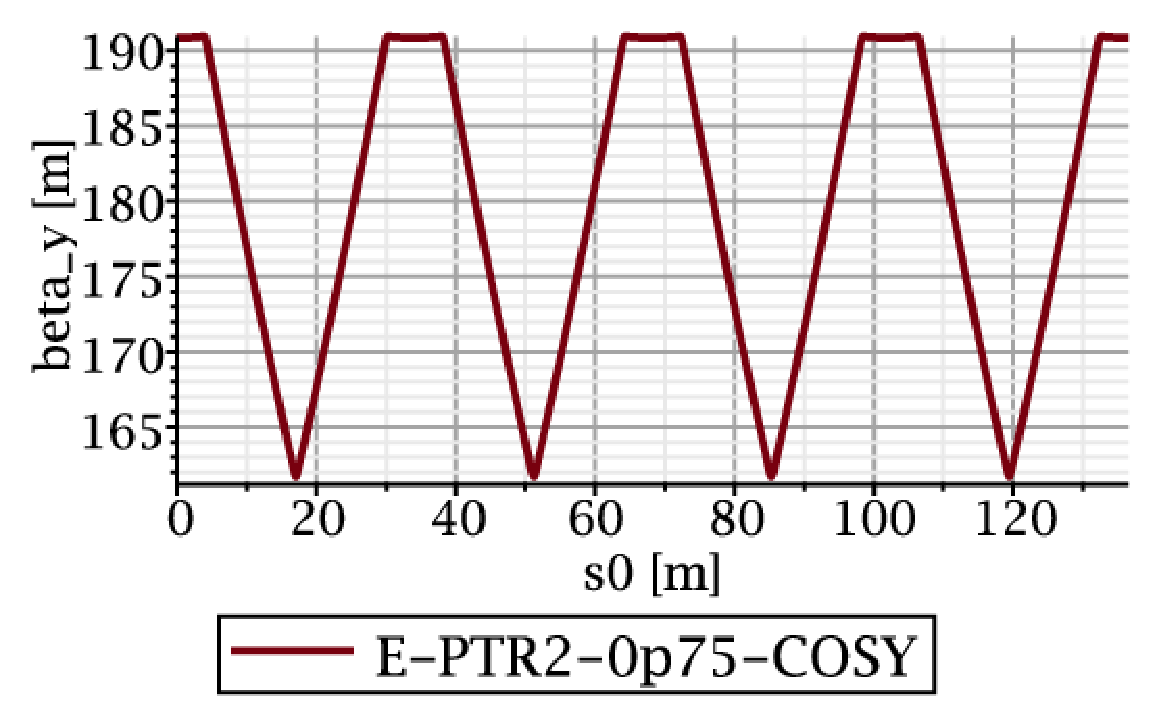
\includegraphics[scale=0.40]{pdf/E-PTR2-0p75-COSY-MAPLE-betay.pdf}
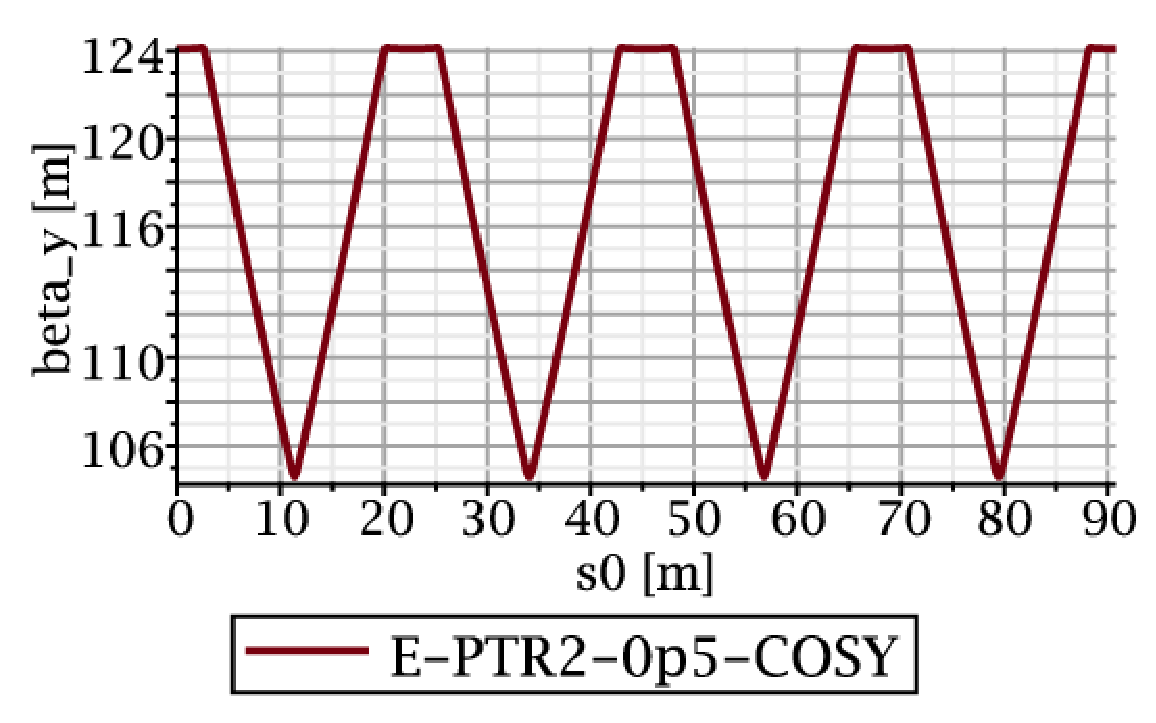
\includegraphics[scale=0.40]{pdf/E-PTR2-0p5-COSY-MAPLE-betay.pdf}
\caption{$\beta_y(s)$ calculated by MAPLE linearized  theory for 
the {\tt E-PTR2} rings.}
\label{fig:E-PTR2-MAPLE-betay}
\end{minipage}
\end{figure}
%

%
\begin{figure}[htbp]
\begin{minipage}[b]{0.45\linewidth}
\centering
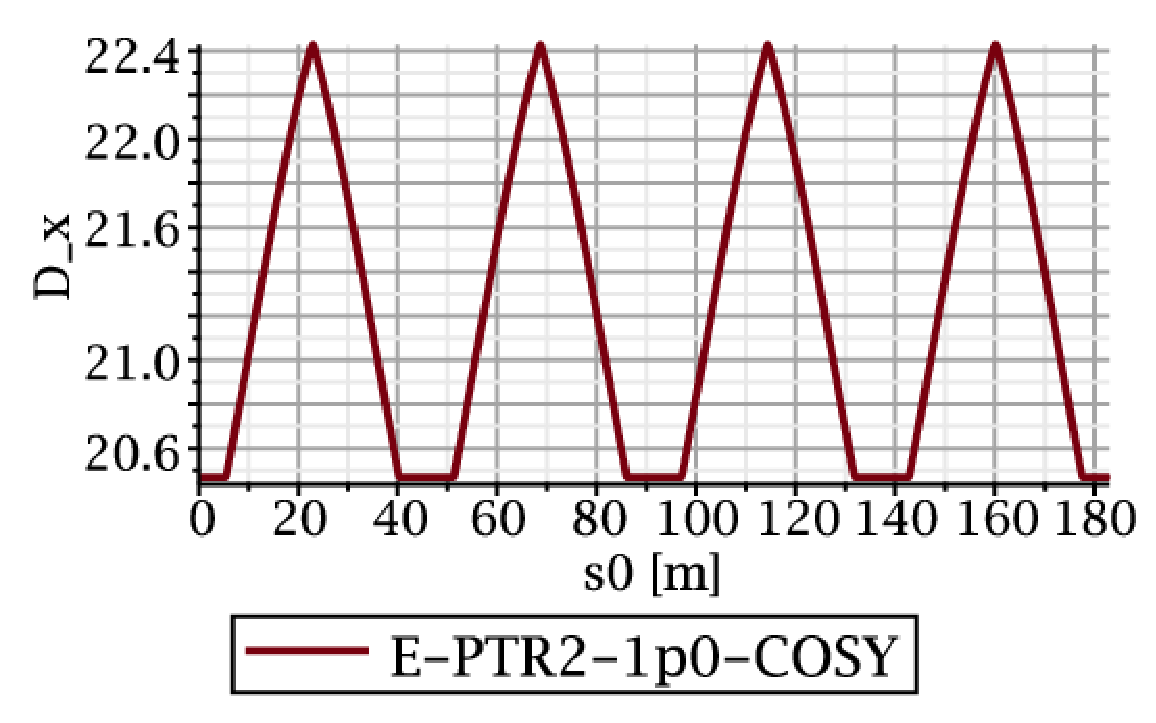
\includegraphics[scale=0.4]{pdf/E-PTR2-1p0-COSY-MAPLE-dispersion.pdf}
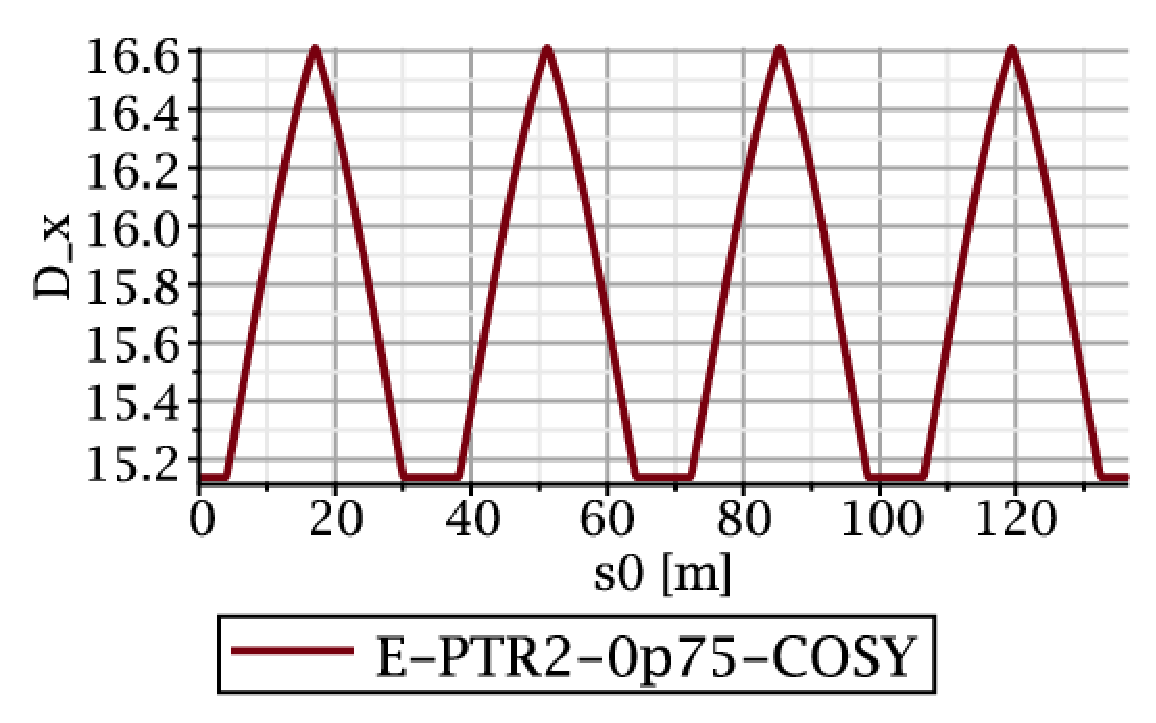
\includegraphics[scale=0.4]{pdf/E-PTR2-0p75-COSY-MAPLE-dispersion.pdf}
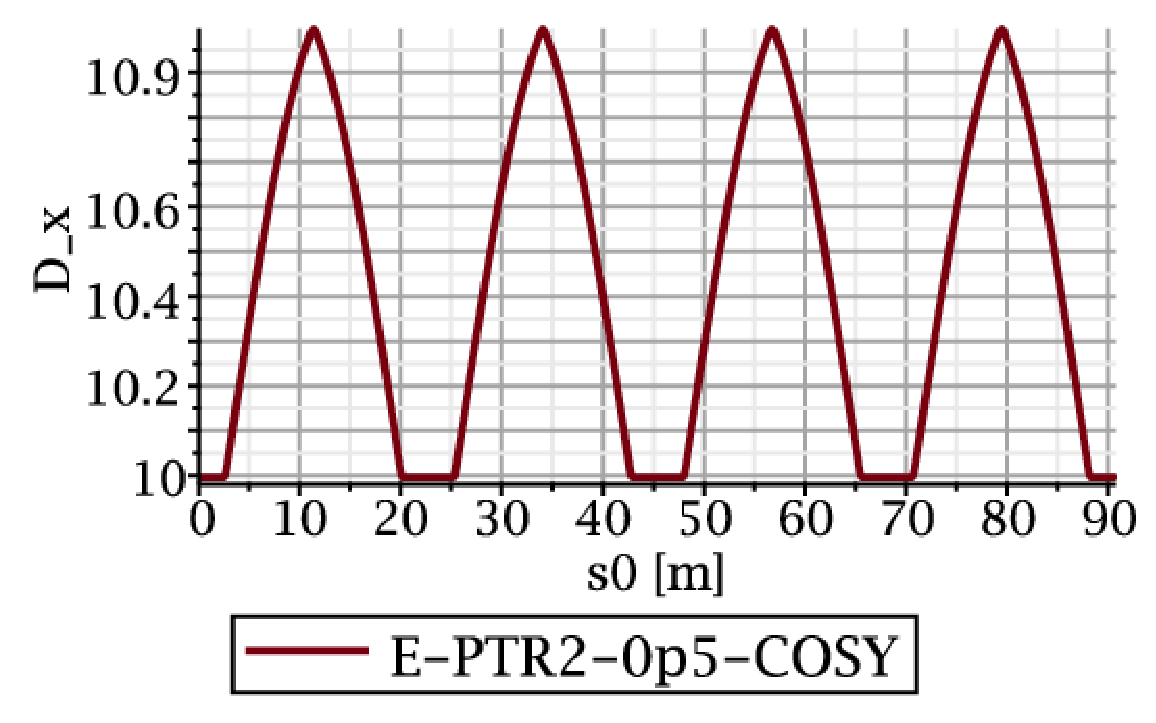
\includegraphics[scale=0.4]{pdf/E-PTR2-0p5-COSY-MAPLE-dispersion.pdf}
\caption{\label{fig:E-PTR2-MAPLE-dispersion}$D(s)$ calculated by MAPLE linearized  theory for 
the {\tt E-PTR2} rings.}
\end{minipage}
%
%
\begin{minipage}[b]{0.45\linewidth}
\centering
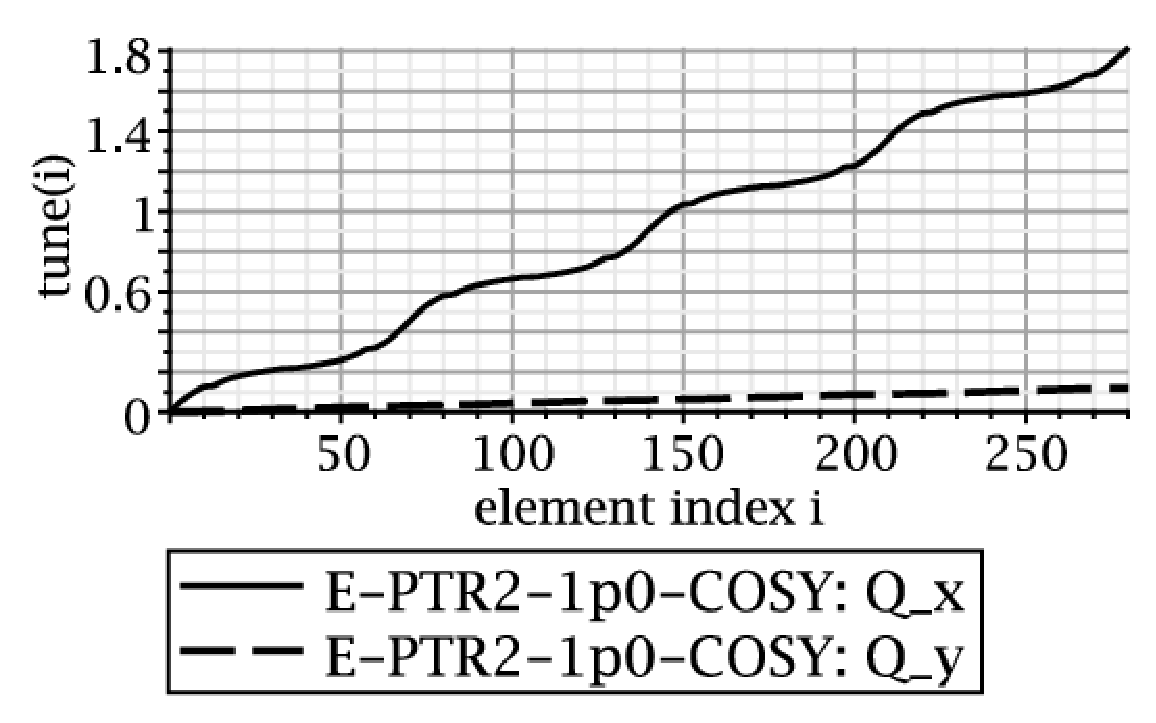
\includegraphics[scale=0.4]{pdf/E-PTR2-1p0-COSY-MAPLE-TuneAdvancex.pdf}
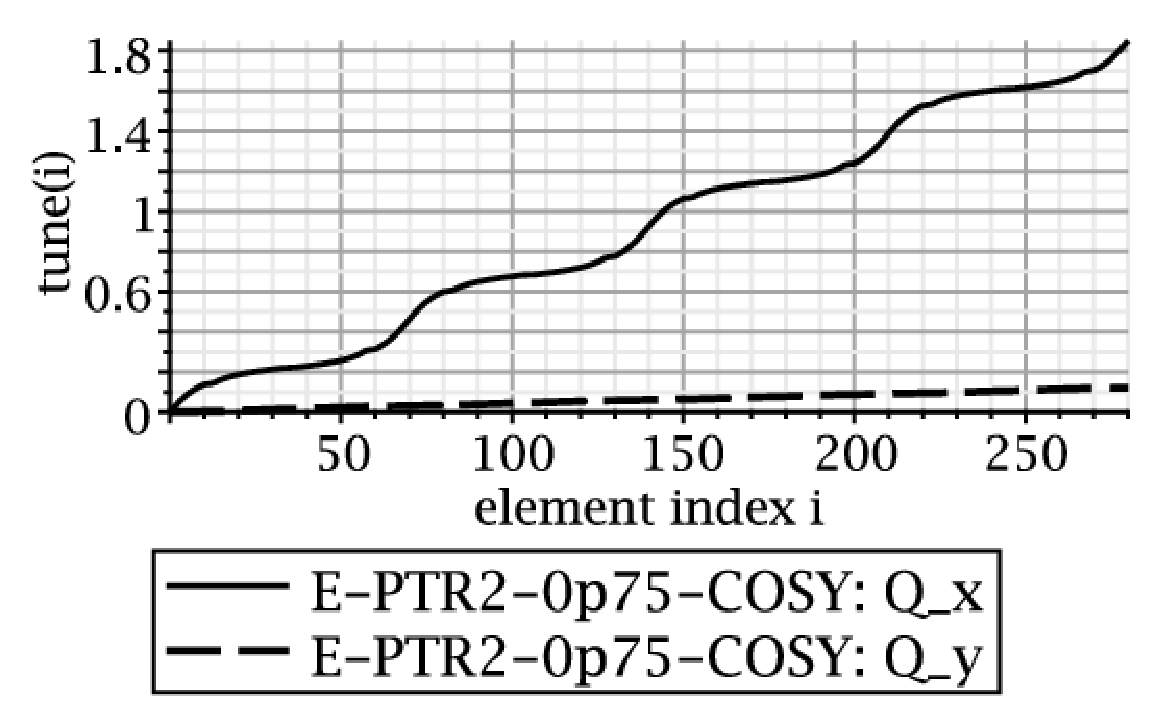
\includegraphics[scale=0.4]{pdf/E-PTR2-0p75-COSY-MAPLE-TuneAdvancex.pdf}
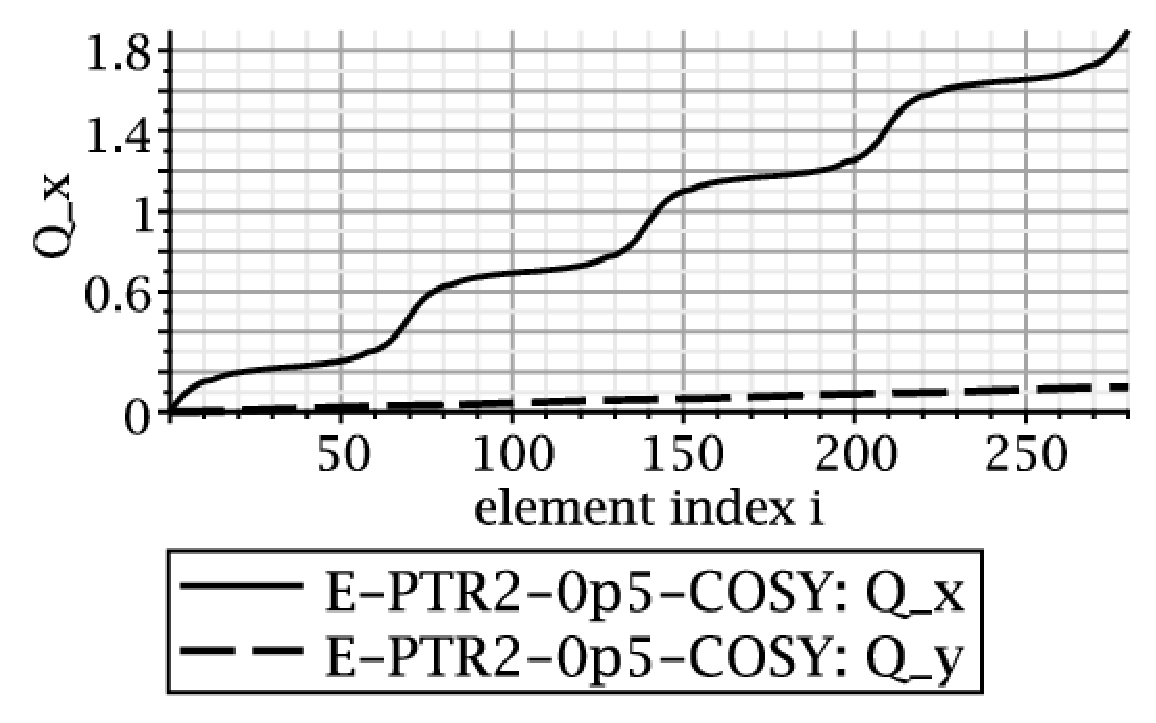
\includegraphics[scale=0.4]{pdf/E-PTR2-0p5-COSY-MAPLE-TuneAdvancex.pdf}
\caption{\label{fig:E-PTR2-MAPLE-TuneAdvance} calculated by MAPLE linearized  theory for 
the {\tt E-PTR2} rings.}
\end{minipage}
\end{figure}
%

%
\begin{table}[hbp]\small %  \footnotesize
\caption{\label{tbl:0p5}MAPLE/ETEAPOT comparisons for 
lattice {\tt E-PTR2-0p5-COSY}} 
\medskip
\centering
\begin{tabular}{|c|c|c|c|c|}           \hline
parameter            & parameter name         & unit & ETEAPOT [-0.032] &    MAPLE      \\ \hline
super-periodicity    &  $N_{\rm S}$             &     &      4       &       4       \\
bend radius          &  {\tt r0}              &  m   &    10.0     &     10.0      \\
long straight length &  {\tt llstot}          &  m   &     6.0     &      6.0      \\
half bend per cell   &  $\Theta=\pi/N_{\rm S}$ &  r    &  0.785398   & 0.785398      \\
half bend length     & {\tt leh}              &  m   &   3.92699   &  3.92699      \\
circumference        & $\mathcal{C}$          &  m   &   90.832    &  90.832       \\
quad strengths       & $qF,qD$                & 1/m  & 0.01, -0.01 & 0.01, -0.01   \\ 
(alternating) field index &  $m$              &      &  $\pm0.002$ & $\pm0.002$    \\  \hline
electric field, 30\,MeV p & $E$                    & MV/m &   5.91      &   5.91        \\
electrode voltages   & $V$                    & KV   & $\pm$206.7  & $\pm$206.7     \\
electrode separation & $gap$                  & cm   &     7       &      7        \\  \hline
horz beta, min/max   & $\beta_x$              &  m   & 1.919, 40.0  & 1.04, 39.5   \\ 
vert beta, min/max   & $\beta_y$              &  m   & 90.2, 129.0  & 104.6, 124.9 \\ 
dispersion, max,min  & $D_x$                  &  m   &              & 10.00, 10.99 \\
horizontal tune      &  {\tt Qx}              &      &   1.833      &    1.898     \\ 
vertical tune        &  {\tt Qy}              &      &   0.1320     &    0.1247    \\
\hline
\end{tabular}
% \end{table}
%
% \begin{table}[hbp]% 
\caption{\label{tbl:0p75}MAPLE/ETEAPOT comparisons for 
lattice {\tt E-PTR2-0p75-COSY}} 
\medskip
\centering
\begin{tabular}{|c|c|c|c|c|}           \hline
parameter            & parameter name         & unit & ETEAPOT [-0.032] &    MAPLE      \\ \hline
super-periodicity    &  $N_{\rm S}$            &      &      4        &       4       \\
bend radius          &  {\tt r0}              &  m   &    15.4      &    15.4       \\
long straight length &  {\tt llstot}          &  m   &   8.932      &  8.932        \\
half bend per cell   &  $\Theta=\pi/N_{\rm S}$ &  r    &  0.785398    & 0.785398      \\
half bend length     & {\tt leh}              &  m   &   6.047      &  6.047        \\
circumference        & $\mathcal{C}$          &  m   & 136.49       & 136.49         \\
quad strengths       & $qF,qD$                & 1/m  & 0.0065, -0.0065 & 0.0065, -0.0065  \\ 
(alternating) field index &  $m$              &      &  $\pm0.002$  & $\pm0.002$    \\  \hline
electric field, 30\,MeV p& $E$                  & MV/m &  3.836       &  3.836       \\
electrode voltages   & $V$                    & KV   & $\pm$134.2   & $\pm$134.2  \\
electrode separation & $gap$                  & cm   &     7        &      7        \\  \hline
horz beta, min/max   & $\beta_x$              &  m   & 3.809, 46.5  & 3.183, 47.43  \\ 
vert beta, min/max   & $\beta_y$              &  m   &   149, 204.0 & 161.7, 190.8  \\ 
dispersion, max,min  & $D_x$                  &  m   &              &  15.2, 16.6    \\
horizontal tune      &  {\tt Qx}              &      &  1.776       &  1.851        \\ 
vertical tune        &  {\tt Qy}              &      &  0.1237      & 0.1214        \\
\hline
\end{tabular}
% \end{table}
%
% \begin{table}[hbp]% 
\caption{\label{tbl:1p0}MAPLE/ETEAPOT comparisons for 
lattice {\tt E-PTR2-1p0-COSY}} 
\medskip
\centering
\begin{tabular}{|c|c|c|c|c|}           \hline
parameter            & parameter name         & unit & ETEAPOT [-0.032] &    MAPLE      \\ \hline
super-periodicity    &  $N_{\rm S}$             &     &      4       &       4       \\
bend radius          &  {\tt r0}              &  m   &   21.0      &      21.0      \\
long straight length &  {\tt llstot}          &  m   &  11.760     &  11.760        \\
half bend per cell   &  $\Theta=\pi/N_{\rm S}$ &  r    &  0.785398   & 0.785398      \\
half bend length     & {\tt leh}              &  m   &  8.247      &  8.247        \\
circumference        & $\mathcal{C}$          &  m   &   183.0     &  183.0        \\
quad strengths       & $qF,qD$                & 1/m  & 0.00476, -0.00476 & 0.00476, -0.00476 \\ 
(alternating) field index &  $m$              &      &  $\pm0.002$ & $\pm0.002$    \\  \hline
electric field, 30\,MeV p & $E$                  & MV/m &  2.813      &  2.813              \\
electrode voltages   & $V$                    & KV   & $\pm$98.45  & $\pm$98.45    \\
electrode separation & $gap$                  & cm   &     7       &      7        \\  \hline
horz beta, min/max   & $\beta_x$              &  m   & 5.898, 5.642 & 5.061, 55.08   \\ 
vert beta, min/max   & $\beta_y$              &  m   & 203.6, 281.8 &  220.7, 259.5  \\ 
dispersion, max,min  & $D_x$                  &  m   &             &  20.5, 22.4   \\
horizontal tune      &  {\tt Qx}              &      &  1.7390     &    1.8163    \\ 
vertical tune        &  {\tt Qy}              &      &  0.1193     &    0.1196    \\
\hline
\end{tabular}
\end{table}
%

\clearpage 

\begin{thebibliography}{99}
\bibitem{CYR}
F. Abusaif, et al., \emph{Storage Ring to Search for Electric Dipole Moments 
of Charged Particles: Feasibility Study,} 
ArXiv: 1912.07881v2 [hep-ex], 2019

\bibitem{Lebedev}
V. Lebedev, \emph{Limitations on an EDM Ring Desin,} EDM collaboration meetings, 
Forschenszentrum Juelich, November 10-11, 2014, and March 13, 2015

\bibitem{BNL-Electic-Analogue}
R. Talman and J. Talman, \emph{Electric dipole moment planning with a resurrected 
BNL Alternating Gradient Synchrotron electron analog ring}, PRST-AB, 18, 
074004, 2015

\bibitem{ETEAPOT}
R. Talman and J. Talman, \emph{ETEAPOT: symplectic orbit/spin tracking code for 
all-electric storage rings,} PRST-AB, 18, 074003, 2015

\bibitem{TEAPOT}
L. Schachinger and R. Talman, \emph{TEAPOT: A Thin-element accelerator program
for optics and tracking,} Particle Accelerators, {\bf 22}, p35, 1987

\bibitem{TEAPOT2}
R. Hinkins, L. Schachinger, and R.Talman, \emph{Synchrotron Oscillations in the SSC with TEAPOT,}
Proceedings of 1986 Snowmass Meeting. SSC-N-217, July, 1986
 
\bibitem{TEAPOT3}
A. Chao et al., \emph{Optimization of the Cell Lattice Parameters for the SSC}, SSC-SR-1024, October 15, 1986

\bibitem{FreqDomain}
R. Talman, \emph{Frequency domain storage ring method for electric dipole moment 
measurement,} arXiv:1508.04366-[physics.acc-ph], 2015

\bibitem{EDM-Challenge}
R. Talman, \emph{The Electric Dipole Moment Challenge,} IOP Publishing, 2017

\bibitem{DoublyMagic}
R. Talman, \emph{A doubly-magic storage ring EDM measurement  method,} 
arXiv:1812.05419-[physics.acc-ph], 2018

\bibitem{RIST-Prospects}
R. Talman, \emph{Prospects for Electric Dipole Moment Measurement Using Electrostati
Accelerators,} in RIST Volume 10, \emph{The Future of Acxcelerators, } A. Chao 
and W. Chou editors, 2019

\end{thebibliography}

\appendix
\section{Lattice description files}
\subsection{E-PTR2-0p75-COSY-con-sl4.xml}
\begin{verbatim}
<xsl:transform version="1.0" xmlns:xsl="http://www.w3.org/1999/XSL/Transform"
    xmlns:xsi="http://www.w3.org/2001/XMLSchema-instance" xmlns:saxon="http://icl.com/saxon"
    xmlns:math="http://exslt.org/math" extension-element-prefixes="saxon math">
    <xsl:variable name="pi" select="3.14159265359"/>
    <xsl:variable name="twopi" select="2*$pi"/>
    <xsl:variable name="tiny" select="0.0000000001"/>
    <xsl:variable name="mcsq" select="0.93827231"/>
    <xsl:variable name="G" select="1.7928474"/>
    <xsl:variable name="c" select="299792458.0"/>
    <xsl:variable name="g" select="2*$G + 2"/>
    <xsl:variable name="R_NOMINAL" select="15.4"/>
    <xsl:variable name="L_LONG_STRAIGHT" select="0.58*$R_NOMINAL"/>
    <xsl:variable name="N_SUPER" select="4"/>
    <xsl:variable name="M_NOMINAL" select="0.002"/>
    <xsl:variable name="TWEAK_LENGTHS" select="1.0"/>
    <xsl:variable name="K0" select="0.030"/>
    <xsl:variable name="Escr0" select="$mcsq + $K0"/>
    <xsl:variable name="gamma0" select="$Escr0 div $mcsq"/>
    <xsl:variable name="p0c" select="math:sqrt($Escr0*$Escr0 - $mcsq*$mcsq)"/>
    <xsl:variable name="beta0" select="$p0c div $Escr0"/>  
    <xsl:variable name="m_in" select="4*$M_NOMINAL div $N_SUPER"/>
    <xsl:variable name="Nsl" select="4"/>
    <xsl:variable name="thetah" select="$pi div $N_SUPER div 2"/>
    <xsl:variable name="thetahsl" select="$pi div $N_SUPER div 2 div $Nsl"/>

    <xsl:variable name="etaE" select="1.0"/>
    <xsl:variable name="etaM" select="(1.0-$etaE)"/>
    <xsl:variable name="r0" select="$R_NOMINAL*$TWEAK_LENGTHS"/>
    <xsl:variable name="leh" select="$thetah*$r0"/>
    <xsl:variable name="lehsl" select="$thetah*$r0 div $Nsl"/>

    <xsl:variable name="lss" select="0.8*$TWEAK_LENGTHS"/>
    <xsl:variable name="lssh" select="$lss div 2"/>
    <xsl:variable name="lssq" select="$lss div 4"/>
    <xsl:variable name="llstot" select="$L_LONG_STRAIGHT*$TWEAK_LENGTHS"/>
    <xsl:variable name="llsh" select="($llstot - $lss) div 2"/>
    <xsl:variable name="llshsl" select="($llstot - $lss) div 2 div 4"/>
    <xsl:variable name="lq" select="$lss div 4"/>
    <xsl:variable name="lqh" select="$lq div 2"/>
    <xsl:variable name="qFh" select="-0.01 div $TWEAK_LENGTHS * 10.0 div $R_NOMINAL"/>
    <xsl:variable name="qDh" select=" 0.01 div $TWEAK_LENGTHS * 10.0 div $R_NOMINAL"/>
    <xsl:variable name="totalstraight" select="$N_SUPER*($llstot + $lss)"/>
    <xsl:variable name="circumference" select="2*$pi*$r0 + $totalstraight"/>
    <xsl:variable name="gBy2" select="0.035"/>
    <xsl:variable name="rfvolt" select="0.000001"/>
    <xsl:variable name="rfharmon" select="1"/>
    <xsl:variable name="rflag" select="0.5"/>
    <xsl:variable name="Trev0" select="$circumference div $beta0 div $c"/>
</xsl:transform>
\end{verbatim}
\subsection{E-PTR2-0p75-COSY-nocon-sl4.xml}
\begin{verbatim}
<xsl:transform version="1.0" xmlns:xsl="http://www.w3.org/1999/XSL/Transform"
    xmlns:xsi="http://www.w3.org/2001/XMLSchema-instance" xmlns:saxon="http://icl.com/saxon"
    xmlns:math="http://exslt.org/math" extension-element-prefixes="saxon math">
    <xsi:elements>
        <element name="mbegin" type="marker"/>
        <element name="mend" type="marker"/>
        <element name="mPeriod" type="marker"/>
        <element name="mhalf" type="marker"/>
        <element name="mQD" type="marker"/>
        <element name="mQF" type="marker"/>

        <element name="RF1" type="rfcavity" l="$tiny">
            <mfield volt="$rfvolt" harmon="$rfharmon" lag='$rflag'/>
        </element> 
        
        <element name="Dlshsl" type="drift" l="$llshsl"/>
        <element name="Dssq" type="drift" l="$lssq"/>
         
        <element name="QFh" type="quadrupole" l="$lqh">
            <mfield a="0" b="$qFh"/>
        </element>
        
        <element name="QDh" type="quadrupole" l="$lq">
            <mfield a="0" b="$qDh"/>
        </element>
        
        <element name="BhMisl" type="sbend" l="$lehsl">
            <mfield a="0" b="concat($etaE*$thetahsl,' ',$m_in*$etaE*$thetahsl)"/>
        </element>

        <element name="BhPlsl" type="sbend" l="$lehsl">
            <mfield a="0" b="concat($etaE*$thetahsl,' ',-$m_in*$etaE*$thetahsl)"/>   
        </element>
                
    </xsi:elements>
    <!--  -->
    <xsi:sectors>

        <sector name="lsin">
            <frame ref="Dlshsl"/>
            <frame ref="Dlshsl"/>
            <frame ref="Dlshsl"/>
            <frame ref="Dlshsl"/>
            <frame ref="Dssq"/>
            <frame ref="mQF"/>
            <frame ref="QFh"/>
            <frame ref="mQF"/>
            <frame ref="mQF"/>
            <frame ref="QFh"/>
            <frame ref="mQF"/>
            <frame ref="Dssq"/>
        </sector>

        <sector name="PM">
            <frame ref="BhPlsl"/>
            <frame ref="BhPlsl"/>
            <frame ref="BhPlsl"/>
            <frame ref="BhPlsl"/>
            <frame ref="BhMisl"/>
            <frame ref="BhMisl"/>
            <frame ref="BhMisl"/>
            <frame ref="BhMisl"/>
        </sector>
        
        <sector name="QDQD">
            <frame ref="Dssq"/>
            <frame ref="mQD"/>
            <frame ref="QDh"/>
            <frame ref="mQD"/>
            <frame ref="QDh"/>
            <frame ref="mQD"/>
            <frame ref="mQD"/>
            <frame ref="QDh"/>
            <frame ref="mQD"/>
            <frame ref="QDh"/>
            <frame ref="mQD"/>
            <frame ref="Dssq"/>
        </sector>

        <sector name="MP">
            <frame ref="BhMisl"/>
            <frame ref="BhMisl"/>
            <frame ref="BhMisl"/>
            <frame ref="BhMisl"/>
            <frame ref="BhPlsl"/>
            <frame ref="BhPlsl"/>
            <frame ref="BhPlsl"/>
            <frame ref="BhPlsl"/>
        </sector>
  
      <sector name="lsout">
            <frame ref="Dssq"/>
            <frame ref="mQF"/>
            <frame ref="QFh"/>
            <frame ref="mQF"/>
            <frame ref="mQF"/>
            <frame ref="QFh"/>
            <frame ref="mQF"/>
            <frame ref="Dssq"/>
            <frame ref="Dlshsl"/>
            <frame ref="Dlshsl"/>
            <frame ref="Dlshsl"/>
            <frame ref="Dlshsl"/>
        </sector>

        <sector name="period">
            <frame ref="lsin"/>
            <frame ref="PM"/>
            <frame ref="QDQD"/>
            <frame ref="MP"/>
            <frame ref="lsout"/>
        </sector>
        
        <sector name="ring">
            <frame ref="mbegin"/>
            <frame ref="mPeriod"/>
            <frame ref="period"/>
            <frame ref="mPeriod"/>
            <frame ref="period"/>
            <frame ref="mPeriod"/>
            <frame ref="mhalf"/>
            <frame ref="mPeriod"/>
            <frame ref="period"/>
            <frame ref="mPeriod"/>
            <frame ref="period"/>
            <frame ref="mPeriod"/>
            <frame ref="mend"/>
        </sector>
    </xsi:sectors>
</xsl:transform>
\end{verbatim}
\end{document}

